\documentclass[]{book}
\usepackage{lmodern}
\usepackage{amssymb,amsmath}
\usepackage{ifxetex,ifluatex}
\usepackage{fixltx2e} % provides \textsubscript
\ifnum 0\ifxetex 1\fi\ifluatex 1\fi=0 % if pdftex
  \usepackage[T1]{fontenc}
  \usepackage[utf8]{inputenc}
\else % if luatex or xelatex
  \ifxetex
    \usepackage{mathspec}
  \else
    \usepackage{fontspec}
  \fi
  \defaultfontfeatures{Ligatures=TeX,Scale=MatchLowercase}
  \newcommand{\euro}{€}
\fi
% use upquote if available, for straight quotes in verbatim environments
\IfFileExists{upquote.sty}{\usepackage{upquote}}{}
% use microtype if available
\IfFileExists{microtype.sty}{%
\usepackage{microtype}
\UseMicrotypeSet[protrusion]{basicmath} % disable protrusion for tt fonts
}{}
\usepackage[margin=1in]{geometry}
\usepackage{hyperref}
\PassOptionsToPackage{usenames,dvipsnames}{color} % color is loaded by hyperref
\hypersetup{unicode=true,
            pdftitle={Ernest iFire Lee's Journal - Chibifire},
            pdfauthor={K. S. Ernest (iFire) Lee},
            pdfborder={0 0 0},
            breaklinks=true}
\urlstyle{same}  % don't use monospace font for urls
\usepackage{natbib}
\bibliographystyle{apalike}
\usepackage{longtable,booktabs}
\usepackage{graphicx,grffile}
\makeatletter
\def\maxwidth{\ifdim\Gin@nat@width>\linewidth\linewidth\else\Gin@nat@width\fi}
\def\maxheight{\ifdim\Gin@nat@height>\textheight\textheight\else\Gin@nat@height\fi}
\makeatother
% Scale images if necessary, so that they will not overflow the page
% margins by default, and it is still possible to overwrite the defaults
% using explicit options in \includegraphics[width, height, ...]{}
\setkeys{Gin}{width=\maxwidth,height=\maxheight,keepaspectratio}
\setlength{\parindent}{0pt}
\setlength{\parskip}{6pt plus 2pt minus 1pt}
\setlength{\emergencystretch}{3em}  % prevent overfull lines
\providecommand{\tightlist}{%
  \setlength{\itemsep}{0pt}\setlength{\parskip}{0pt}}
\setcounter{secnumdepth}{5}

%%% Use protect on footnotes to avoid problems with footnotes in titles
\let\rmarkdownfootnote\footnote%
\def\footnote{\protect\rmarkdownfootnote}

%%% Change title format to be more compact
\usepackage{titling}

% Create subtitle command for use in maketitle
\newcommand{\subtitle}[1]{
  \posttitle{
    \begin{center}\large#1\end{center}
    }
}

\setlength{\droptitle}{-2em}
  \title{Ernest `iFire' Lee's Journal - Chibifire}
  \pretitle{\vspace{\droptitle}\centering\huge}
  \posttitle{\par}
  \author{K. S. Ernest (iFire) Lee}
  \preauthor{\centering\large\emph}
  \postauthor{\par}
  \predate{\centering\large\emph}
  \postdate{\par}
  \date{2017-12-03}


% Redefines (sub)paragraphs to behave more like sections
\ifx\paragraph\undefined\else
\let\oldparagraph\paragraph
\renewcommand{\paragraph}[1]{\oldparagraph{#1}\mbox{}}
\fi
\ifx\subparagraph\undefined\else
\let\oldsubparagraph\subparagraph
\renewcommand{\subparagraph}[1]{\oldsubparagraph{#1}\mbox{}}
\fi

\usepackage{booktabs}
\usepackage{amsthm}
\makeatletter
\def\thm@space@setup{%
  \thm@preskip=8pt plus 2pt minus 4pt
  \thm@postskip=\thm@preskip
}
\makeatother

\begin{document}
\maketitle

{
\setcounter{tocdepth}{1}
\tableofcontents
}
\chapter{Blog}\label{intro}

This is chibifire.com where I post my research notes.

\section{Godot art pipeline investigations
\#1}\label{godot-art-pipeline-investigations-1}

 Sunday, December 3, 2017 10:25:36 AM

Asked in the Godot discord about how people were doing the Godot 3.0 3d
art import workflow.

I was trying to import assets from sketchfab (gltf2 format) and a lot of
the work was fixing textures - material mappings

Steps:

\begin{itemize}
\tightlist
\item
  Disable ect2 compression in Godot 3 Editor.
\item
  Convert from FBX using
  \url{https://github.com/pissang/qtek-model-viewer} - 3D model viewer
  with high quality rendering
\item
  Import gltf2
\item
  Fix material mapping
\end{itemize}

\section{Godot}\label{godot}

 Sun, 13 Aug 2017 16:26:52 +0000

I have been investigating godot. It's a 3d game engine that has support
for physically based rendering.

\chapter{Physics in Super Jet Racing - 29 June
2015}\label{physics-in-super-jet-racing---29-june-2015}

\emph{This is a guest article from ReactorScram.}

I'm ReactorScram, I've been doing Ludum Dare since April 2013. This game
is a followup to my LD27 entry, ``Jet Racing''. People complained it was
too 2D so I made 3D physics for this ``Super Jet Racing''.

In my game, you race a hovercar. Originally I wanted to make a game like
F-Zero where the car sticks to the track and is able to hang
upside-down. I could still do this, but it seemed making a big F-Zero
track would be time-consuming and hard to test.

The level is only about half-done, but I imagine it existing inside a
stadium, like they race monster trucks in. There's concrete barriers
marking the edges of the track, and right before the start / finish line
is a one-kilometer wall, angled at 85 degrees, with a checkpoint at the
top. The car has a high thrust-weight ratio, and the player is expected
to drive straight up the wall, pass the checkpoint, and fall back down.

As my physics method in my custom engine, I used discrete collision
detection and explicit Euler integration. Discrete collision detection
means I was too lazy to do continuous collision.

Every frame I check whether the car is inside a triangle, then I push it
out. I do this up to 20 times, in case the car is in multiple triangles.

Apparently, you must use an epsilon for this, otherwise the car may keep
pushing itself out of a triangle that it's not really in. That one
triangle would eat up all the collision resolve steps and leave nothing
for the other triangles. During testing, this manifested as: running
into a wall and the car would fall through the ground.

When I push the car out of a triangle, I also zero its velocity along
the normal of the triangle to simulate an inelastic collision.

There wasn't any issues with penetration other than falling through the
ground.

Near the beginning, I had implemented the AABB check before the triangle
check, so briefly the car was not colliding with inclined planes
properly.

I didn't encounter problems with the car rocketing into the air. Even
though I'm using explicit Euler, the simulation is very simple and it
doesn't seem to explode. I'm also doing physics at 120 FPS so tunneling
has not been an issue. Once I saw it seem to teleport, but it hasn't
happened since then. I don't know what it was.

It helps that the track doesn't have any sharp edges where the car might
get caught. There's also no other moving objects than the car, although
I'd like to add enemy cars, ghost cars or multiplayer someday.

My method is notable because it was hand-written in Lua over the course
of a few days.

Cowritten by Ernest `iFire' Lee

\section{Additional Notes}\label{additional-notes}

Recently Devlin noticed the car's turning looks too ``tight'', that it
does not drift enough. I had already allowed the car to drift in theory.

Every frame, car's sideways velocity is measured and friction is applied
to it. If the velocity is small, it will be set to zero, otherwise it
will decrease linearly from the friction. The friction was changed so
that the threshold for setting the sideways velocity to zero is higher
than the amount by which the velocity linearly decreases.

This should simulate a car's tires having high static friction but low
kinetic friction. (Even though it's a hovercraft). During a normal turn,
the car will grip the road, but if the centrifugal force of the turn
becomes too high, the grip will suddenly break and the car will drift.
There needs to have some different kinds of curves in the track to test
whether this feels right.

For the car to drive up walls, its rotation needs to be changed so the Z
vector of the car matches the normal of the wall. As part of the
collision detection, a list of normals is created of any walls or floors
(the engine doesn't differentiate them) that the car is touching. The
game chooses the normal closest to the car's previous Z vector and
assumes that the car should drive along that surface. Afterwards, the
game interpolates the car's quaternion so that the car will gradually
rotate to drive along the wall / floor.

As a result of this, the car pitches back when it drives off of a ramp.
If the car jumps off a ramp and turn 90 degrees left or right, the car
will be turning within the plane of the ramp, and the camera will show
the world tilted slightly sideways as the car drifts through the air.

The car is modelled as a sphere of diameter 5 meters. Maybe this is the
right ballpark for a racing hovercar, because Formula One cars are 5
meters long. To make sure that the car wouldn't tunnel through anything,
I went to Wikipedia and measured the speed / body length ratios of
Formula One cars and SR-71s.

I don't remember the exact numbers, but in 1 / 120th of a second, an F1
car only moves roughly 80 cm. An SR-71 moves a number of meters, but
SR-71s are also 107 feet long.

In Super Jet Racing, the car peaks around 3 meters per frame, which I
think is 1200 scale kilometers per hour. I might need to change the
graphics to make it feel faster.

\subsection{Grid System}\label{grid-system}

To accomodate large tracks, I use a 3D grid. When the track is loaded,
the game iterates over every triangle, placing it into grid buckets
based on its AABB. When the game is running, it uses the same function
to place the car into grid buckets. Then for collision detection, it
only considers triangles within the car's grid buckets.

The current track has about 1,400 triangles so it is useless to check
triangles that are nowhere near the player.

A benchmark was setup that spawns the car, then idles for 100,000
physics frames.

Grid on: - 18.7 seconds - less than 0.2 milliseconds per physics frame,
including the time needed to set up the grid.

Grid off: - 2 minutes and 43 seconds: - 1.63 milliseconds per frame.

Right now the game is not hurting for milliseconds, but on a weaker CPU,
or on a bigger track, or with multiple players, the grid will be a
necessity.

\chapter{Pirate Nomnoml}\label{pirate-nomnoml}

 Sunday, April 16, 2017 4:11:05 PM

\href{http://nomnoml.com}{Nomnoml} makes uml diagrams.

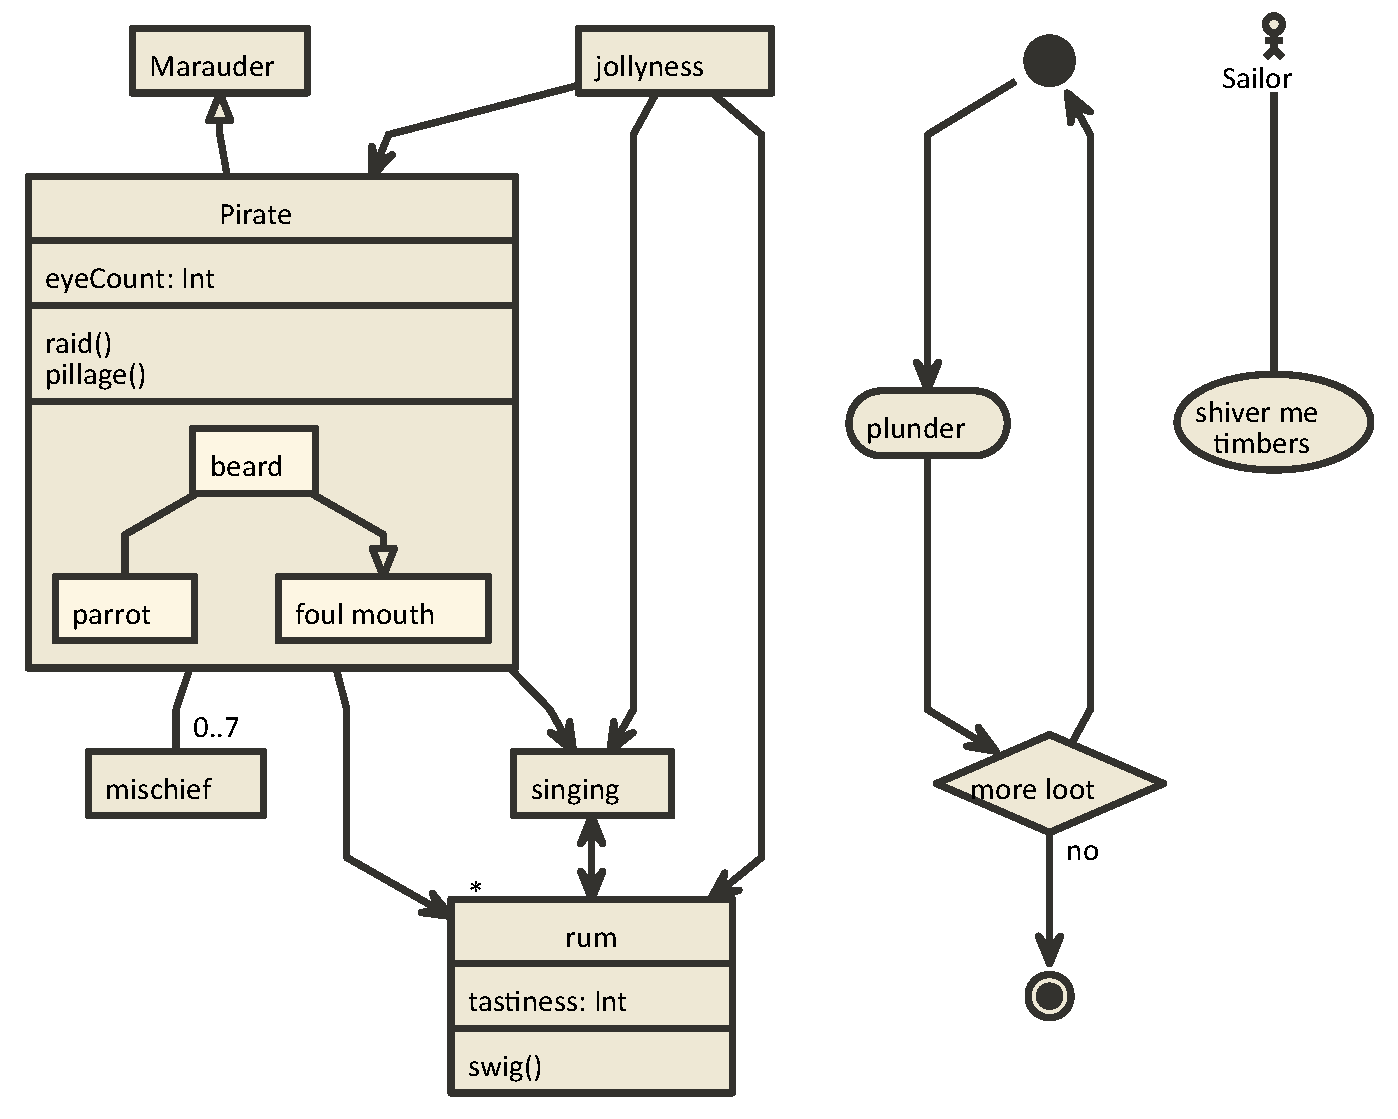
\includegraphics{Image/Pirate.nomnoml.pdf}

\chapter{Portfolio}\label{portfolio}

\section{Current Projects:}\label{current-projects}

\textbf{Squad - Offworld Industries}:

\includegraphics{Image/Squad_(videogame)_2016_frontcover.png}

Programmer

\section{Previous Projects:}\label{previous-projects}

\subsection{Heavy Gear Assault - Mektek Studos /
Stompybot:}\label{heavy-gear-assault---mektek-studos-stompybot}

\includegraphics{Image/HeavyGearAssaultPromoImage.jpg}

Systems Professional

\subsection{Jam at iamagamer:}\label{jam-at-iamagamer}

Penny Farthing by Team Penny

For the \texttt{@iamagamer} game jam, it's a game about a little girl
full of mirth and ready to get her meadow frolic on.

Credits

Michelle Clough Michelle Buch Nick Irvine Shih Oon Liong Ernest Lee

\url{http://jam.iamagamer.ca/submissions/80-penny-farthing}

\bibliography{book.bib,packages.bib}

\end{document}
